\begin{itemize}
	\item Magnetische Momente durch Elektronen in Atomen
	\item Magnetische Momente (MMe) des Elektronensystems von Atomen als Ursache der magnetischen Wechselwirkung
	\item Je nach Art der WW zwischen Materie und Magnetfeldern lassen sich die Materialien in die folgenden "Klassen" unterteilen:
	\begin{itemize}
		\item Paramagnetische
		\item Diamagnetische
		\item Ferromagnetische
		\item Antiferromagnetische
		\item Ferrimagnetische
	\end{itemize}
	Materialien
\end{itemize}
Wie äußert sich entsprechend Magnetismus?\\
Experiment: Spule mit Luft: $ \vec{B} = \vec{B_0} $\\
\indent Spule mit Eisenkern: $ \vec{B} >> \vec{B_0} $ ; $ \vec{B} \approx 4...5 \times \vec{B_0} $
\subsection{Betrachte Magnetischesmoment eines kreisenden geladenen Teilchens}
\begin{center}
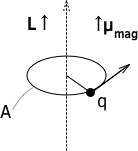
\includegraphics[width=0.2\linewidth]{skizzen/17/17B01}
\end{center}
\begin{align*}
\mu_{mg} = I \cdot A = \left( \frac{q}{T} \right)  \cdot (\pi r^2) &= \frac{1}{2} \cdot q \cdot \omega r^2\\
&= \frac{q}{2m} \cdot |\vec{L}|\\
\text{Es gilt: } \vec{\mu}_{mg} = \frac{q}{2m} \cdot \vec{L}
\end{align*}
Für Elektronen im Atom:
$$ \boxed{\vec {\mu}_{mg} = \frac{-e}{2m_e} \cdot \vec{L} } $$
$ \Rightarrow $ MM durch Bahndrehimpuls!\\
Bohr'sches Atommodell: Drehimpuls ist quantisiert $$ |\vec{L}| = n\cdot \hbar \hspace{5mm} \left( \hbar = \frac{h}{2\pi}\right)  $$\\
kleinster Wert: $ n=1 $ : $$ \mu = -\frac{e}{2m_e}\cdot \hbar = \mu_{Bohr} = \SI{-9,13e-24}{\ampere\meter^2} $$\\
$ \mu_{Bohr} $ : Bohr'sches Magnetton $$ \underline{\underline{\Rightarrow \mu = n \cdot \mu_{Bohr}}} $$ \\
Gyromagnetisches Verhältnis (g-Faktor):
$$ g= \frac{(\mu/|\vec{L}|)}{\frac{1}{2}\frac{e}{m_e}} = 1 \text{ für Bahnelektronen} $$ \\
Zusätzlich berücksichtigen: Eigendrehimpuls des Elektrons (Spin) $ S=\frac{1}{2} \hbar $ (Quantenmechanik) \\
Bei der Berechnung des zugehörigen MM tritt ein zusätzlicher Faktor auf: $ g_S $ :
$$ \vec{\mu}_S = -q_S \cdot \frac{e}{2m_e} \cdot \vec{S} $$
$$ g_S \approx 2,0 $$ \\
$ \Rightarrow $ gesamtes MM eines $ e^- $ ist die Summe aus Beitrag von $ \vec{L} $ und $ \vec{S}$. \\
$ \Rightarrow $ gesamtes MM eines Atoms ist $ \sum $ der MM alle einzelnen $ e^- $ !\\
$ \Rightarrow $ Je nach Elektronkonfiguration (Besetzung der verschiedenen Schalter) ist Kompensation möglich \\
$ \Rightarrow $ Komplett gefüllte Schalen liefern keinen Beitrag zum MM! \\
$ \Rightarrow $ Materialien wie He, Ne, Ar, ... sind nicht magnetisierbar \\
$ \Rightarrow $ Diese Effekte bestimmen die "Magnetisierung" des Materials! \\ \break
Äußeres Feld $ \vec{B}_0 $:
$$ \vec{B} = \vec{B}_0 + \overbrace{\mu_0 \vec{M}}^{Magnetisierung} $$
$ \vec{M} $ : mittleres magnetisches Moment/Volumen
$$ \vec{M} = n\cdot \underbrace{<\vec{\mu}_{mg}>}_{\text{mittl. MM/Atom(Molekül)}} $$ \begin{flushright}
	\emph{n}: Dichte der Atome (Moleküle)
\end{flushright}
$$ \boxed{\vec{B} = \vec{B}_0 + \mu_0 \cdot \vec{M}} $$
Anschauliche Erklärung: Ampere: "Atomare Ringströme"
\begin{center}
	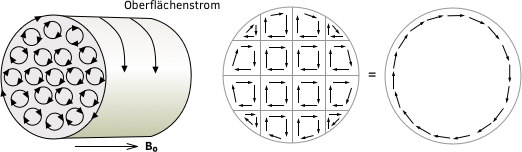
\includegraphics[width=0.7\linewidth]{skizzen/17/17B02}
\end{center}
Naives Bild: "Ausrichtung der Elementarmagnete" (..Schale)\\ \break

\noindent Magnetische Feldstärke: $ \vec{H} $ \\
Im Vakuum/Luft: $ \vec{B}_0 = \mu_0 \cdot \vec{H} $\\
Mit Materie: 
\begin{align*}
\vec{B} &= \vec{B}_0 + \mu_0 \cdot \vec{M} = \mu \cdot \vec{H} \\
&\mu_0 \cdot \vec{H} + \mu_0 \vec{M} \\
\Rightarrow &= \mu_0 \cdot \vec{H} (1+\underset{\text{magnetische Suszeptibilität}}{X_m})\\
&=\mu_0 \cdot \mu_r \cdot \vec{H}\\
\mu_r(1+X_m) \hspace{2mm}&\text{relative Permeabilität}\\
\mu = \mu_0\mu_r \hspace{2mm} &\text{Permeabilität}
\end{align*}

\begin{center}
	$ X_m > 0 $ \hspace{5mm} : \textcolor{green}{Paramagnet $ \bullet $}\\
	$ X_m < 0 $ \hspace{5mm} : \textcolor{blue}{Diamagnet $ \bullet $}
\end{center}
\begin{center}
	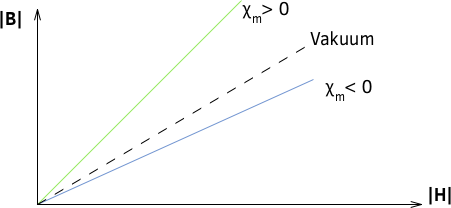
\includegraphics[width=0.5\linewidth]{skizzen/17/17B03}
\end{center}
Experiment: Materie im inhomogenen Magnetfeld
\begin{center}
	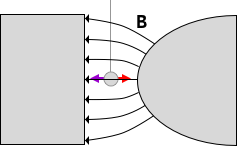
\includegraphics[width=0.5\linewidth]{skizzen/17/17B04}
\end{center}
Paramagnet: wird in inhom. $ \vec{B} $-Feld hineingezogen\\
Diamagnet: wird aus $ \vec{B}_{inhom} $ heraus-gedrängt\\
Ferromagnet: Wie Paramagnet, aber \underline{viel} stärker\\
\begin{itemize}
	\item Diamagnetismus\\
	\begin{itemize}
		\item Störung der $ e^- $-Bahnen durch äußeres Feld
		\item Verursacht kleine MMe, die $ \uparrow \downarrow $ zu $ \vec{B}_0 $ sind.
		$$ \vec{M}  \uparrow \downarrow  \vec{B}_0 \Rightarrow \mathcal{X}_m <0 \text{ !} $$
		\item Tritt bei allen Materialien auf, wird aber fast immer durch Paramagnetismus überlagert.
	\end{itemize}
	\item Paramagnetismus\\
	$ \exists $ pemanente MMe aus Bahn- und Spinmagnetismus der Valenzelektronen, die im äußeren $ \vec{B} $-Feld entgegen der thermischen Bewegung ausgerichtet werden:
	$$ \vec{M} \uparrow\uparrow \vec{B}_0 \Rightarrow \mathcal{X}_m > 0 \text{ !}$$ 
	Für kleine Magnetfelder: $ |\vec{M}| \sim |\vec{B}_0|/T$ \\
	Für große Felder (und/oder kleine Temperaturen; $ \mu_{mag} \cdot B_0 >> k_BT $) komplette Ausrichtung, dann $ |\vec{M}| = |\vec{M}_S|_{\text{ $ \leftarrow $  Sättigungsmagnetisierung}} $\\
	\begin{center}
		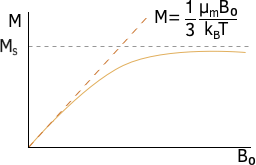
\includegraphics[width=0.5\linewidth]{skizzen/17/17B05}
	\end{center}
	Curie-Gesetz: $ M = \frac{1}{3} \frac{\mu_{mg}\cdot B_0}{k_BT} \cdot M_S $ \hspace{1cm} ($ \mathcal{X}_m \sim T^{-1}$)
	\item Ferromagnetismus\\
	Hier: WW der MMe untereinander ("Spin$ \cdot $Spin-WW")\\
	Beitrag zur freien Energie: \\
	$$ E = -\frac{1}{2} \cdot \overset{\text{Austauschkonstante}}{J} \underset{\text{Gitterplätze}}{\sum_{i,j}} S_i S_j $$
	$$ S_{i,j} = \pm \frac{1}{2}\text{ , } +\frac{1}{2}: \hspace{3mm}\uparrow \hspace{3mm} \text{ , } -\frac{1}{2}: \hspace{3mm}\textbf{$ \downarrow $} \hspace{3mm} MM$$\\
	$ \Rightarrow $ Kompetitiv: Energieminimierung/Entropiemaximierung !\\
	$ \Rightarrow $ Benachbarte MMe "wollen" parallel stehen!
	$ \Rightarrow $ $ \mathcal{X}_m =\mathcal{X}_m (\vec{B}_0) $ \\
	$ \Rightarrow $ permanente Magnetisierung, wenn Temperatur nicht zu hoch! \\
	$ \Rightarrow $ Parallele Ausrichtung der MMe in mikroskopischem Bereich\\
	\hspace{5mm}"Domänen" (Weiss'sche Bezirke) \hspace{3mm} $ 10^{-8} ... 10^{-12} \text{ m}^3 $ \hspace{2mm},\hspace{2mm} $ 10^{21}...10^{17} \text{ Atome} $
	$ \Rightarrow $ \underline{Barkhausen-Effekt !}
\end{itemize}
\newpage
\begin{itemize}
	\item i Ferromagnetsimus: Mikroskopisch \\
	\begin{center}
		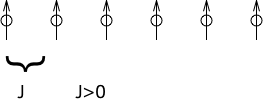
\includegraphics[width=0.5\linewidth]{skizzen/17/17B06}
	\end{center}
	
	Beitrag zur Energie $ E= - \frac{1}{2}J \ds{\sum_{i,j} s_i s_j} \hspace{5mm} s_{i,j} = \pm 1/2 $ \\
	\item ii $ J<0 $ \\
	\begin{center}
		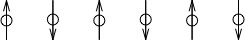
\includegraphics[width=0.5\linewidth]{skizzen/17/17B07}
	\end{center}
	
	Antiferromagnetismus
	Gesamtmagnetisierung $ "0" $
	\item iii
	\begin{center}
		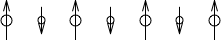
\includegraphics[width=0.5\linewidth]{skizzen/17/17B08}
	\end{center}
	Ferrimagnetismus (nicht verschwindende Gesamtmagnetisierung)
\end{itemize}
$ \Rightarrow $ Ferromagnetische Kopplung $ \Rightarrow $ Domänenstruktur\\ \break
Magnetisierung im äußeren Feld:
\begin{center}
	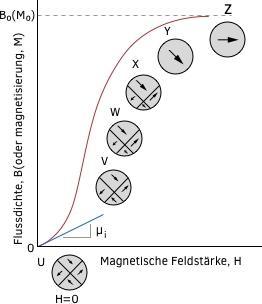
\includegraphics[width=0.5\linewidth]{skizzen/17/17B09}
\end{center}

\begin{enumerate}
	\item Domänenwachstum
	\item Drehung der Magnetisierung
\end{enumerate}

Zu 1. : Kein Kontinuierlicher Prozess, sondern:

\begin{center}
	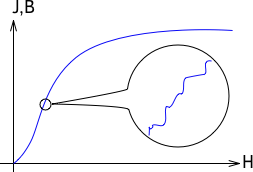
\includegraphics[width=0.5\linewidth]{skizzen/17/17B10}
\end{center}
$ \Rightarrow $ \emph{Barkhausen-Effekt} \\ \break
Energiebilanz (Einfluss der Entropie!): Ferromagnetische Ordnung nicht temperaturstabil, d.h. einer "kritischen Temperatur" (Curie-Temperatur) Übergang zu paramagnetischem Verhalten.\\ \break

$ \boxed{\text{Exp: Drehender Ni.Ring}} $ \\
"Stabilen" ferromagnetische Ordnung:
$ \Rightarrow $ "Arbeit" notwendig, um Magnetisierung aufzuheben (oder: äußeres Feld in Gegenrichtung!)
\begin{center}
	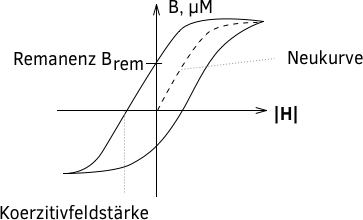
\includegraphics[width=0.5\linewidth]{skizzen/17/17B12}
\end{center}
$ \Rightarrow $ Hysterese \\
Weichmagnetische Stoffe: leicht mangnetisierbar (Kleine Fläche von Hysterese umschlossen)\\
Hartmagnetische Stoffe: schwer magnetisierbar, große Fläche\\
